\chapter{开发环境的配置}
\label{cha:Environment}

在这一章,着重阐述Windows 10环境下开发环境的配置方法。

\section{Mega 2560开发环境}

本节主要叙述了如何烧写Bootloader:需要两块板,Programmer和Target,首先按对应的引脚一一对应连接MISO/MOSI/SCK/Reset/GND/5V,之后给Programmer上传Arduino ISP Skectch,之后选择编程器为Arduino as ISP,烧写引导程序,如果之后要使用ICSP烧Target的程序的话,就点 项目 > 使用编程器上传即可。参考\url{https://www.arduino.cc/en/Hacking/HomePage}。

\subsection{初次使用烧写固件}

在AVR单片机的每次复位时都执行了一段特殊的代码,并使用特定的协议和速度从串行/ USB端口上载了Sketch。如果未检测到连接,则执行将传递到Sketch的代码。

这小段代码(通常为512字节)被称为“Bootloader”,如图~\ref{fig:MemoryMap},它位于微控制器的内存区域中地址空间的末尾,被设计为用于引导,不能重新编程为常规Sketch。

\begin{figure}[htbp]
    \centering
    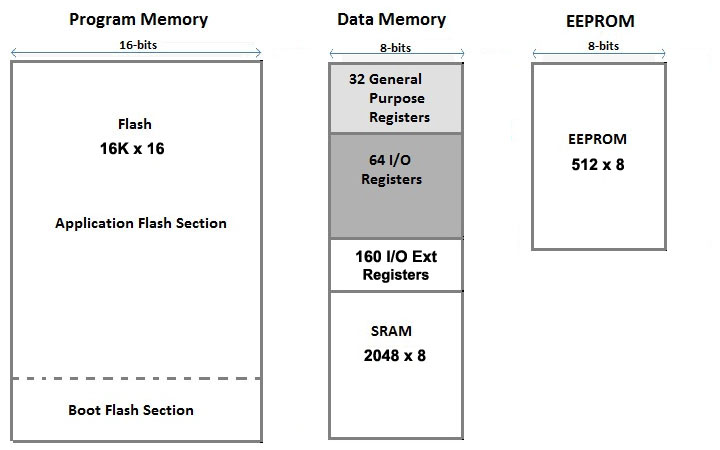
\includegraphics[width=0.5\columnwidth]{MemoryMap.jpg}
    \caption{ATmega328P 内存映射}
    \label{fig:MemoryMap}
\end{figure}

一般来说,微控制器通过编程器被烧写程序(programmer),除非微控制器中有一个固件(firmware),该固件允许无需外部编程器而安装新固件。这种固件称为引导加载程序(bootloader)。新出厂的微控制器内部不含Bootloader,必须要先烧录引导程序

\begin{figure}[htbp]
    \centering
    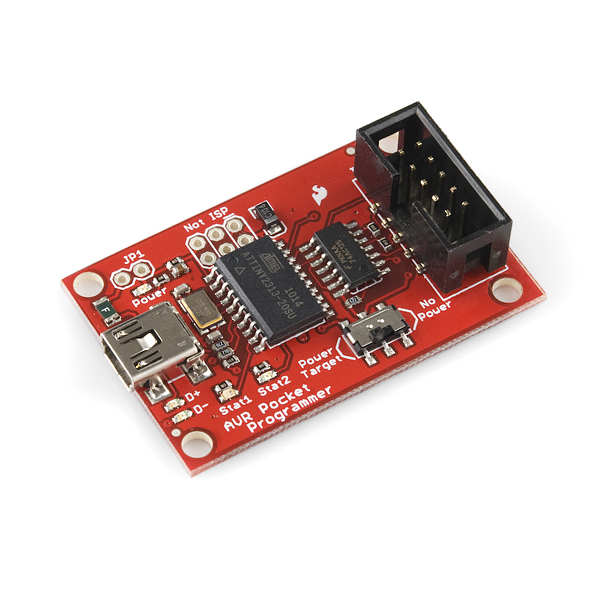
\includegraphics[width=0.5\columnwidth]{Pocket-AVR-Programmer.jpg}
    \caption{Pocket AVR Programmer}
    \label{fig:Pocket-AVR-Programmer}
\end{figure}

烧写Bootloader\footnote{\url{https://www.arduino.cc/en/Hacking/Bootloader}}需要先购买AVR-ISP (in-system programmer,如图~\ref{fig:Pocket-AVR-Programmer}), USBtinyISP 或者自己做一个ParallelProgrammer(并行编程器),这些编程器需要连接到ICSP引脚(如图~\ref{fig:Isp_headers}),同时板子需要通电(USB或者电池都可以)。

\begin{figure}[htbp]
    \centering
    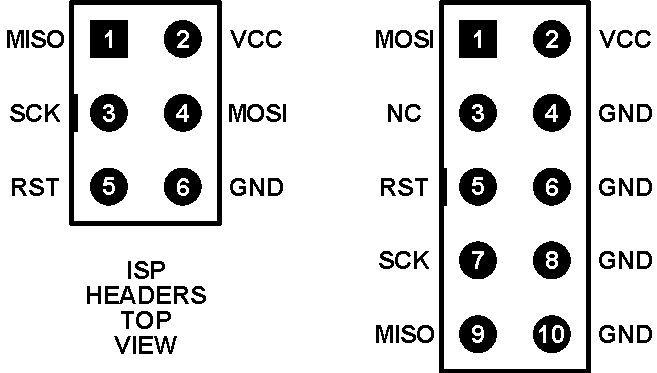
\includegraphics[width=0.5\columnwidth]{Isp_headers.pdf}
    \caption{6- and 10-pin ISP header}
    \label{fig:Isp_headers}
\end{figure}

在Arduino IDE中,确保 Tools > Board 选项是对的(注意要选成目标板Target的型号,比如在本项目中目标板就是Arduino Mega1280 or Mega2560),之后开始 Tools > Burn Bootloader 等待约15秒即可。

也可以使用编程器对应的软件比如AVRISP MkII的AVRStudio进行烧写操作,参考\url{https://www.arduino.cc/en/Hacking/MiniBootloader}。

另外,如果不购买专用的ISP,可以通过一块Arduino Mega 2560 开发板给本项目的电路板烧写程序\footnote{参考\url{https://www.arduino.cc/en/Hacking/Upgrading16U2Due}}。事实上,本项目就是这样给每块芯片烧写引导的。

做法如下:

在Arduino IDE里面打开示例文件 ArduinoISP并烧写到用作烧写器的Arduino上。

在 GND 和 RESET之间连接一个10uF的电容,并将Arduino Uno (or Mega)如表~\ref{tab:ICSP}所示的引脚连接到要烧写芯片的对应ICSP引脚上,如图~\ref{fig:Arduino-Mega-Mega-Sketch}。

% Please add the following required packages to your document preamble:
% \usepackage{booktabs}
\begin{table}[htbp]
    \centering
    \begin{tabular}{@{}llll@{}}
    \toprule
          & Uno & Mega & 16U2 ICSP \\ \midrule
    SCK   & 13  & 52   & 3         \\
    MISO  & 12  & 50   & 1         \\
    MOSI  & 11  & 51   & 4         \\
    Reset & 10  & 10   & 5         \\
    GND   & GND & GND  & 6         \\
    +5V   & 5V  & 5V   & 2         \\ \bottomrule
    \end{tabular}
    \caption{ICSP}
    \label{tab:ICSP}
\end{table}

\begin{figure}[htbp]
    \centering
    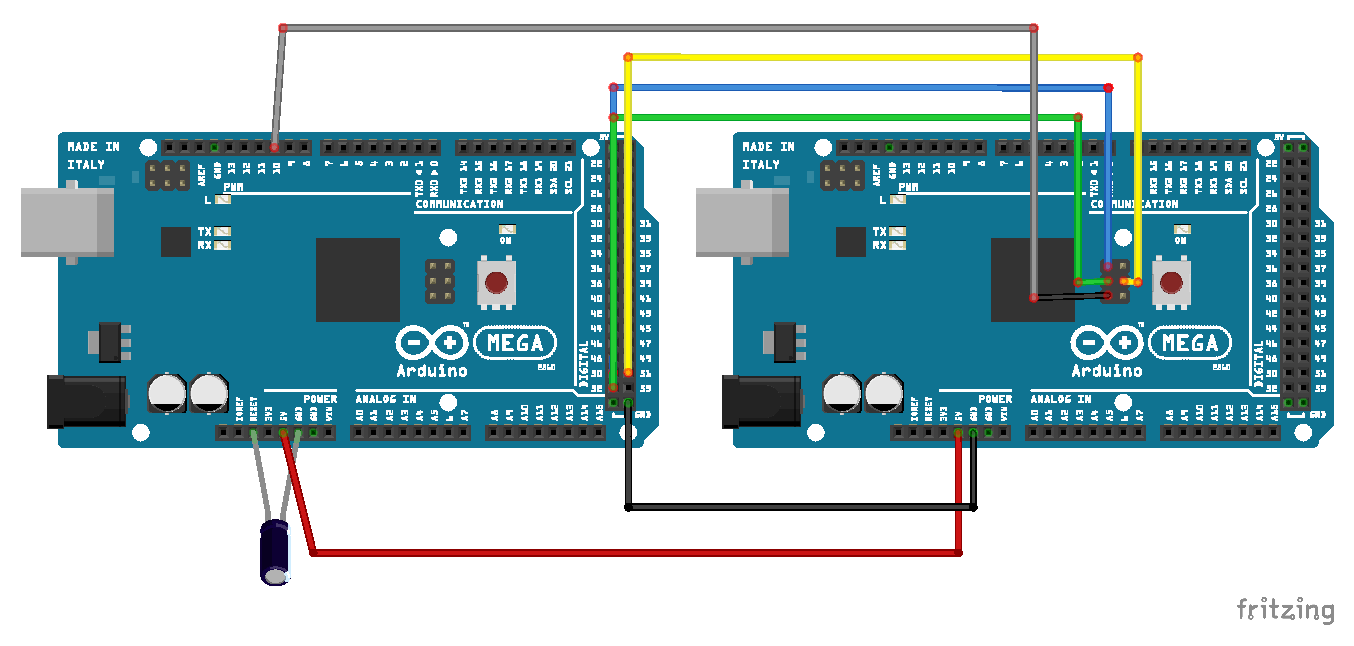
\includegraphics[width=\columnwidth]{Arduino-Mega-Mega-Sketch.pdf}
    \caption{Arduino-Mega-Mega-Sketch}
    \label{fig:Arduino-Mega-Mega-Sketch}
\end{figure}

最后使用avrdude命令进行固件烧写,avrdude 可以在 /path to arduino/arduino.1.8.x/hardware/tools 路径找到。

要烧写进16U2的固件是 .hex 扩展名的二进制文件,首先CMD/Terminal路径设置到avrdude所在的文件夹里,之后运行如下命令:

Windows:

\begin{tcolorbox}
    arduino-1.5.2/hardware/tool> avrdude.exe -C avrdude.conf -c arduino -P /dev/ttyACM0 -b 19200 -p m16u2 -vvv -U flash:w:/home/USER/newFirmware/16u2.hex:i
\end{tcolorbox}

Linux and Mac:

\begin{tcolorbox}
    /home/USER/arduino-1.5.2/hardware/tools\$ ./avrdude -C avrdude.conf -c arduino -P /dev/ttyACM0 -b 19200 -p m16u2 -vvv -U flash:w:/home/USER/newFirmware/16u2.hex:i
\end{tcolorbox}

avrdude参数解释见表~\ref{tab:avrdude}

\begin{table}[htbp]
    \centering
    \begin{tabular}{ll}
    -C avrdude.conf                              & load the configuration file for using the Arduino Uno as programmer       \\
    -c arduino                                   & specify the programmer you want to use                                    \\
    -P /dev/ttyACM0                              & the usb port where the programmer is attached                             \\
    -b 19200                                     & the baudrate                                                              \\
    -p m16u2                                     & the target device you want to program                                     \\
    -vvv                                         & enable the verbose output                                                 \\
    -U flash:w:/home/USER/newFirmware/16u2.hex:i & specify that you want to write (w) the  .hex file inside the flash memory
    \end{tabular}
    \caption{Avrdude parameter explanations}
    \label{tab:avrdude}
\end{table}

只要找到对应的ICSP引脚,烧写ATMega2560和ATmega16U2的操作基本一致。如图~\ref{fig:Arduino-Mega-UNO-Sketch}。

更加具体的解释见\url{https://www.arduino.cc/en/Tutorial/ArduinoISP}

\begin{figure}[htbp]
    \centering
    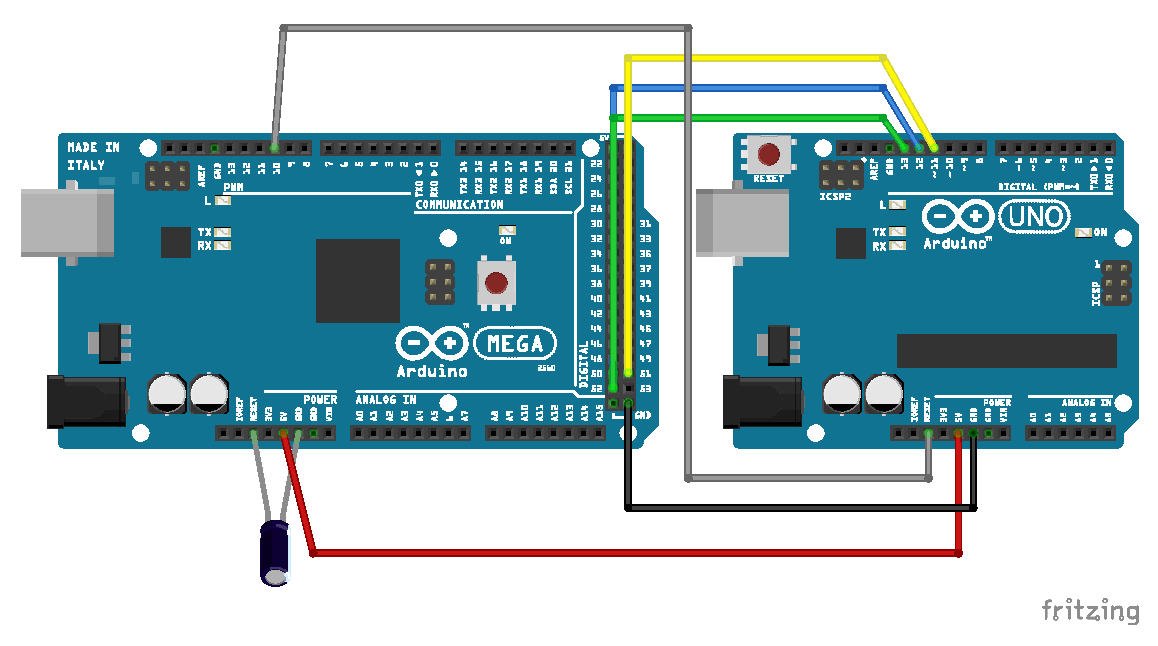
\includegraphics[width=\columnwidth]{Arduino-Mega-UNO-Sketch.pdf}
    \caption{Arduino-Mega-UNO-Sketch}
    \label{fig:Arduino-Mega-UNO-Sketch}
\end{figure}

\subsection{Arduino IDE}

本项目使用的ATmega2560-16AU和ATmega16U2-MU芯片组是Arduino IDE支持的,对应ARDUINO MEGA 2560 REV3开发板,因此,本开发环境将基于Arduino IDE(\url{https://www.arduino.cc/en/Main/Software})进行搭建。

\begin{figure}[htbp]
    \centering
    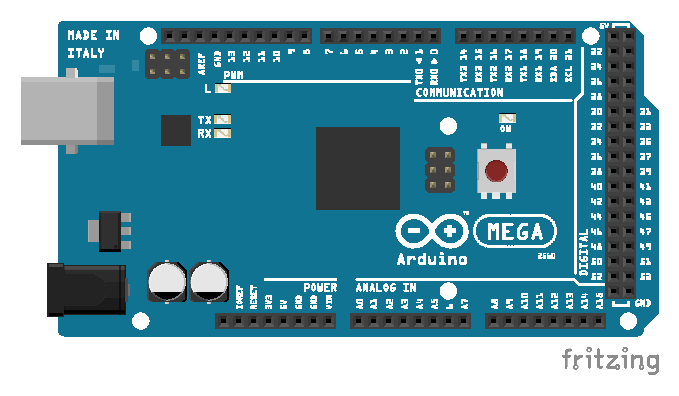
\includegraphics[width=\columnwidth]{Arduino-Fritzing.pdf}
    \caption{Arduino Mega}
    \label{fig:Arduino-Fritzing}
\end{figure}

Arduino集成开发环境(Arduino IDE)包含了一个用于写代码的文本编辑器、一个消息区、一个文本控制台以及一个带有常用功能按钮和文本菜单的工具栏。连接Arduino之后,软件能给所连接的控制板上传程序,还能与控制板相互通信。

使用Arduino软件(IDE)编写的代码被称为项目(sketches),这些项目写在文本编辑器中,以.ino的文件形式保存

IDE UI中上传按钮的作用是编译代码并且上传到选定的控制板中,注意:如果你使用的是专门的编程器,你需要在点击按钮时按住电脑的“shift”键,显示的文字会变成“使用编程器上传”。

在上传之前,需要在 Tools - Board 和 Tools - Port 中选定开发板类型和端口,在本项目中,选择Arduino/Genuino Mega 2560 (Arduino/Genuino Mega 2560
An ATmega2560 running at 16 MHz with auto-reset, 16 Analog In, 54 Digital I/O and 15 PWM.)开发板。

端口在Windows系统中,串口显示为 COM1 或 COM2,USB则显示为COM3及以上,选择对应的端口即可。



\section{ESP 32开发环境配置}

本节阐述搭建 ESP32 硬件开发的软件环境,软件编译和烧写流程\footnote{\url{https://docs.espressif.com/projects/esp-idf/zh_CN/v4.0-rc/get-started/}}如图~\ref{fig:ESP-Need}。

\begin{figure}[htbp]
    \centering
    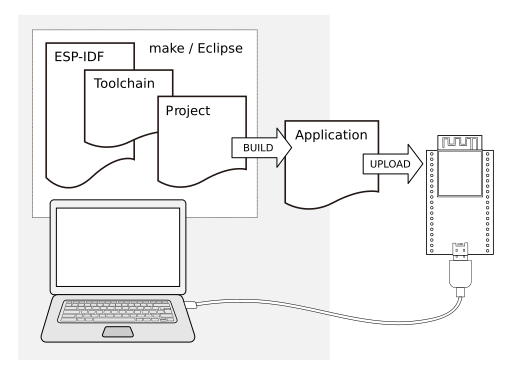
\includegraphics[width=0.6\columnwidth]{ESP-Need.png}
    \caption{ESP32 应用程序开发}
    \label{fig:ESP-Need}
\end{figure}

\subsection{Windows平台ESP-IDF工具链的标准设置}

ESP-IDF 需要安装一些必备工具,才能围绕 ESP32 构建固件,包括 Python、Git、交叉编译器、menuconfig 工具、CMake和 Ninja 编译工具等。

要安装 ESP-IDF 必备工具,最简易的方式是下载 ESP-IDF 工具安装器\footnote{\url{https://dl.espressif.com/dl/esp-idf-tools-setup-2.2.exe}}。

安装器可安装所需的交叉编译器、OpenOCD、cmake 和 Ninja 编译工具,以及一款 mconf-idf 配置工具。此外,本安装器还可在有需要时下载、运行 Python 3.7 和 Git For Windows 的安装器,如图~\ref{fig:IDF-Installer}。

\begin{figure}[htbp]
    \centering
    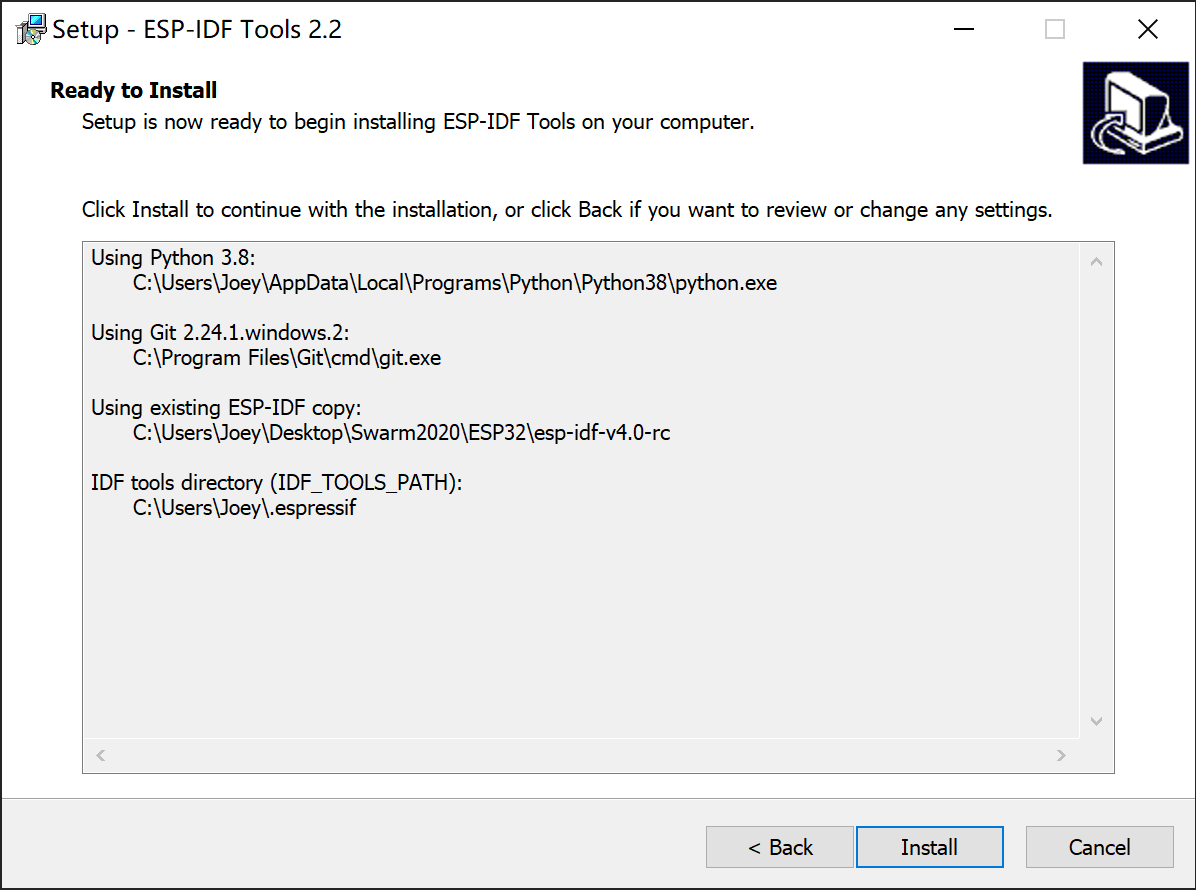
\includegraphics[width=0.7\columnwidth]{IDF-Installer.png}
    \caption{ESP-IDF 工具安装器配置}
    \label{fig:IDF-Installer}
\end{figure}

\subsection{获取 ESP-IDF}

除了工具链,还需要供 ESP32 使用的 API(软件库和源代码),具体请见 ESP-IDF 仓库。

请将 ESP-IDF 下载到本地。

获取本地副本:打开终端,切换到要存放 ESP-IDF 的工作目录,使用 \mintinline{powershell}|git clone| 命令克隆远程仓库:

% \mint{powershell}|git clone -b v4.0-rc --recursive https://github.com/espressif/esp-idf.git|
\begin{tcolorbox}
    git clone -b v4.0-rc --recursive https://github.com/espressif/esp-idf.git
\end{tcolorbox}

GitHub 中”下载 zip 文档”的功能不适用于 ESP-IDF,所以需要使用 git clone 命令。作为备份,可以在没有安装 Git 的环境中下载 Stable version 的 zip 归档文件。直接在\url{https://github.com/espressif/esp-idf/releases/download/v4.0-rc/esp-idf-v4.0-rc.zip}下载并解压。

\subsection{安装 Python 软件包}

如果是使用ESP-IDF工具安装器安装的,此步骤可能已经完成。

ESP-IDF 所需的 Python 软件包位于 IDF-PATH/requirements.txt 中。可以运行以下命令进行安装:

% \mint{powershell}|python -m pip install --user -r $IDFPATH/requirements.txt|

\begin{tcolorbox}
    python -m pip install --user -r IDFPATH/requirements.txt
\end{tcolorbox}

\subsection{编辑环境变量}

如果是使用ESP-IDF工具安装器安装的,此步骤可能已经完成。

需要在用户配置文件中添加 IDF PATH 和 idf.py PATH

使用基于 CMake 的构建系统和 idf.py 工具,用户需修改两处系统环境变量:

\begin{itemize}
    \item IDF\underline{ }PATH 需设置为含有 ESP-IDF 目录的路径
    \item 系统 PATH 变量需包括含有 idf.py 工具的目录
\end{itemize}

如果从未用过 idf.py 命令行工具,而是直接运行 cmake 或通过 IDE 工具运行 cmake,则无需设置 PATH 变量,只需设置 IDF PATH 变量。不过,也可以两个都设置。如果只用过 idf.py 命令行工具,从未直接运行 cmake 或通过 IDE 工具运行 cmake,则无需设置 IDF PATH 变量。idf.py 会搜索自身包含的目录,如果没有发现 IDF PATH,则会自行进行有关设置。

在 Windows 10 操作系统下设置环境变量,用户应在开始菜单下搜索 “Edit Environment Variables”。

在较早版本的 Windows 操作系统下设置环境变量,用户应打开系统控制面板,选择“高级”,找到环境变量按钮。

可以为本台电脑上的“所有用户”或“当前用户”设置环境变量,这取决于其他用户是否也需要使用 ESP-IDF。

点击 New... (新建…) 添加名为 IDF\underline{ }PATH 的新系统变量,具体设置为包含 ESP-IDF 的目录,例如,C:/Users/user-name/esp/esp-idf。

找到 Path 环境变量,双击进行编辑。在末尾添加 ;IDF\underline{ }PATH \backslash tools ,这样就可以通过 Windows 命令窗口运行 idf.py 等其他工具了。

\subsection{开始创建工程}

现在,可以开始准备开发 ESP32 应用程序了。可以从 ESP-IDF 中 examples 目录下的 get-started/hello-world 工程开始。ESP-IDF 编译系统不支持带有空格的路径,可能需要复制到其他目录下再运行。

\subsection{连接设备}

用 USB 线将 ESP32 开发板连接到 PC。如果设备驱动程序没有自动安装,请先确认 ESP32 开发板上的 USB 转串口芯片(或外部转串口适配器)型号,然后在网上搜索对应的驱动程序,并进行手动安装。

CP210x: CP210x USB 至 UART 桥 VCP 驱动程序 \url{https://www.silabs.com/products/development-tools/software/usb-to-uart-bridge-vcp-drivers}

FTDI: FTDI 虚拟 COM 端口驱动程序 \url{https://www.ftdichip.com/Drivers/VCP.htm}

一般情况下,当上述任一 ESP32 开发板与 PC 连接时,对应驱动程序应该已经被打包在操作系统中,并已经自动安装。

现在,将 ESP32 开发板连接到 PC,并查看开发板使用的串口。检查 Windows 设备管理器中的 COM 端口列表。断开 ESP32 与 PC 的连接,然后重新连接,查看哪个端口从列表中消失,然后再次出现。

通常,串口在不同操作系统下显示的名称有所不同:

\begin{itemize}
    \item Windows 操作系统: COM1 等
    \item Linux 操作系统: 以 /dev/tty 开始
    \item MacOS 操作系统: 以 /dev/cu. 开始
\end{itemize}


\subsection{工程配置}

在使用ESP-IDF工具安装器安装的ESP-IDF Command Prompt (cmd.exe)中

Python 2.7 安装程序将尝试配置 Windows,将 .py 文件与 Python 2 关联起来。如果其他程序(比如 Visual Studio Python)曾关联了其他版本 Python,则 idf.py 可能无法正常运行(文件将在 Visual Studio 中打开)。这种情况下,可以选择每次都运行一遍 C:/Python27/python idf.py,或更改 Windows 的 .py 关联文件设置。

如果默认 Python 版本为 3.0 以上,可能需要运行 python2 idf.py。


使用ESP-IDF Command Prompt (cmd.exe) 在/esp/hello world示例工程路径下运行:

\begin{tcolorbox}
    idf.py menuconfig
\end{tcolorbox}

会显示菜单:

\begin{figure}[htbp]
    \centering
    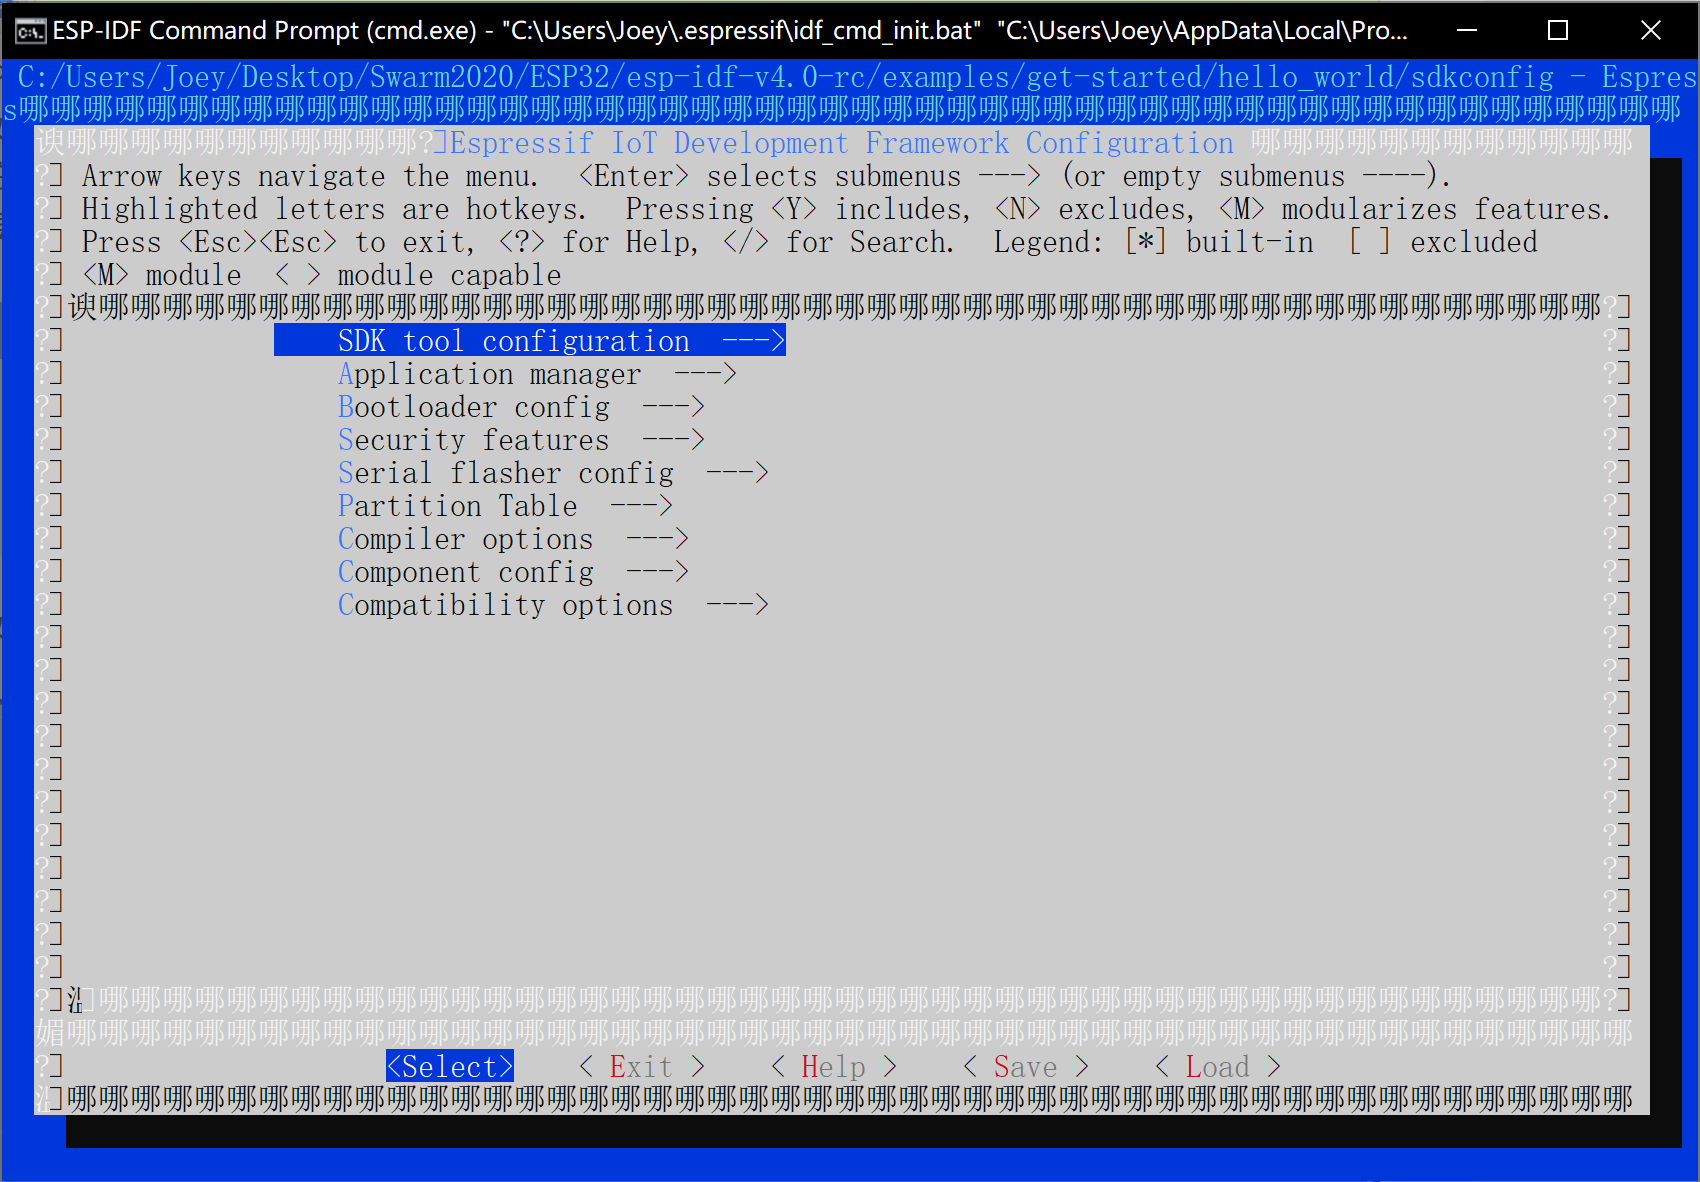
\includegraphics[width=\columnwidth]{ESP-IDF-Config.png}
    \caption{ESP-IDF 设置}
    \label{ESP-IDF-Config}
\end{figure}

\subsection{编译工程}

在ESP-IDF Command Prompt (cmd.exe)中使用以下命令,编译烧录工程:

\begin{tcolorbox}
    idf.py build
\end{tcolorbox}

运行以上命令可以编译应用程序和所有 ESP-IDF 组件,接着生成 bootloader、分区表和应用程序二进制文件。如图~\ref{fig:ESP-IDF-Build}

\begin{figure}[htbp]
    \centering
    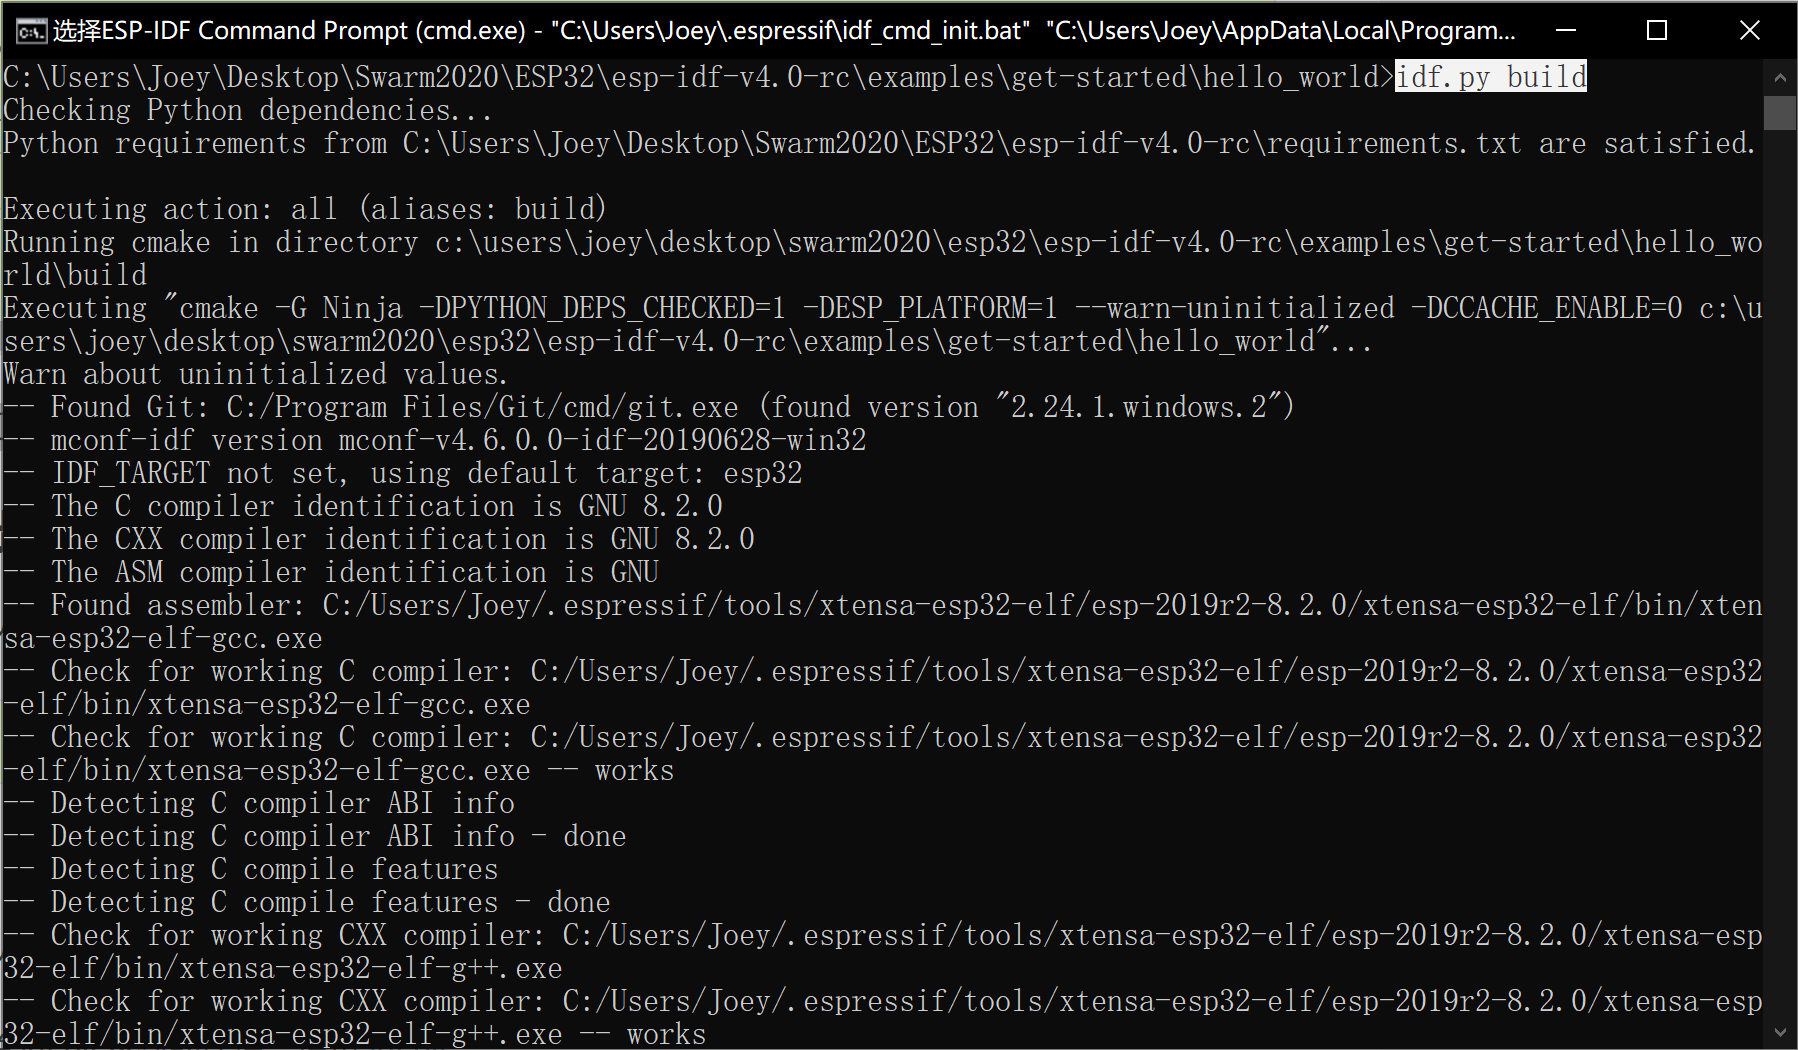
\includegraphics[width=\columnwidth]{ESP-IDF-Build.png}
    \caption{ESP-IDF idf.py build}
    \label{fig:ESP-IDF-Build}
\end{figure}

如果一切正常,编译完成后将生成 .bin 文件。如图~\ref{fig:ESP-IDF-Build-2}

\begin{figure}[htbp]
    \centering
    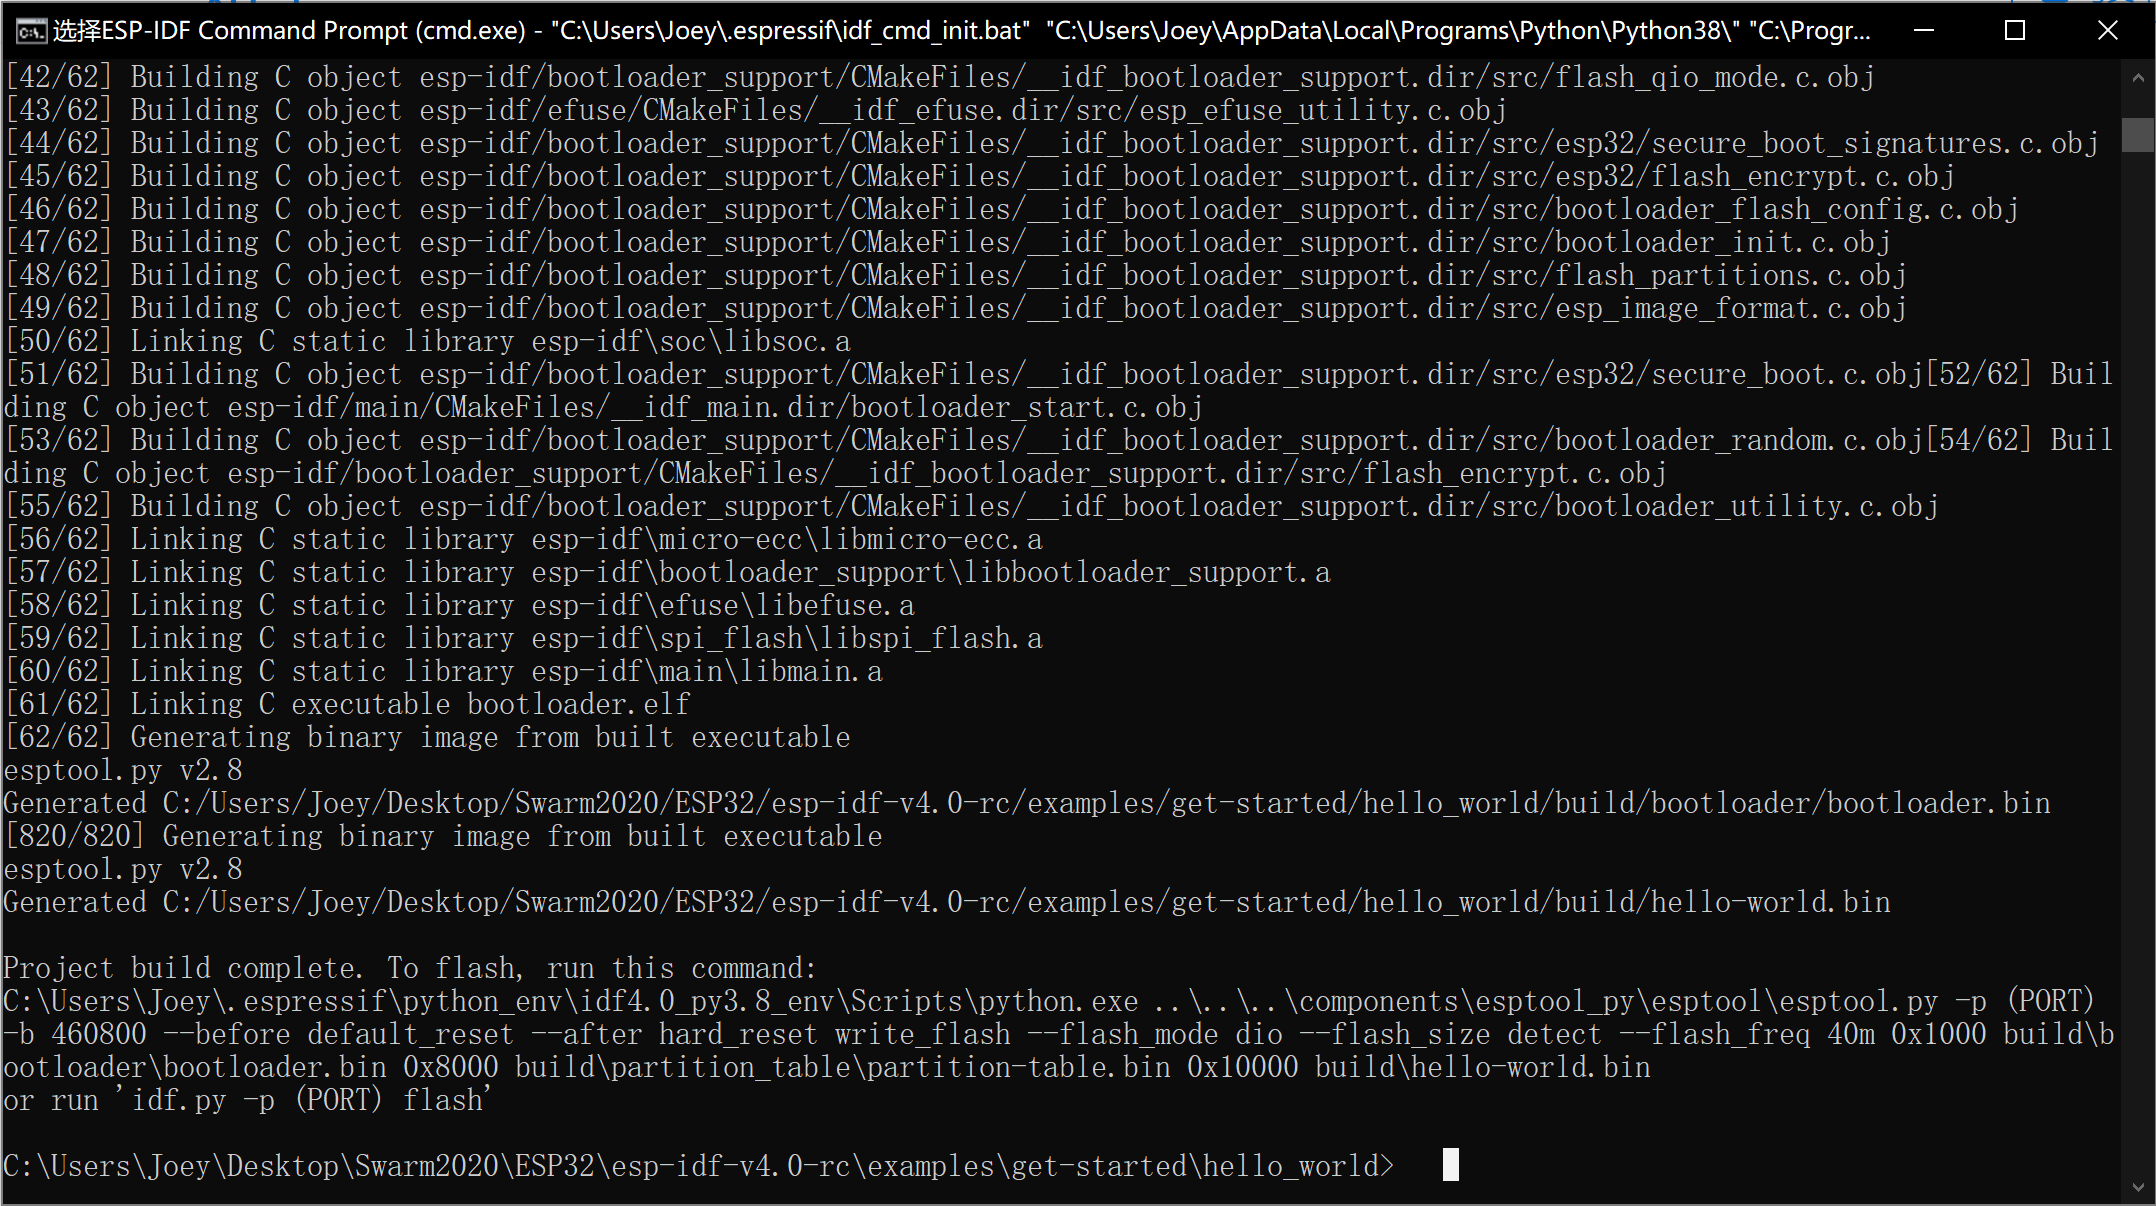
\includegraphics[width=\columnwidth]{ESP-IDF-Build-2.png}
    \caption{ESP-IDF idf.py build}
    \label{fig:ESP-IDF-Build-2}
\end{figure}

\subsection{烧录到设备}

将 PORT 替换为 ESP32 开发板的串口名称,使用以下命令,将刚刚生成的二进制文件烧录至 ESP32 开发板:

\begin{tcolorbox}
    idf.py -p PORT [-b BAUD] flash
\end{tcolorbox}

还可以将 BAUD 替换为希望的烧录波特率。默认波特率为 460800

如果一切顺利,烧录完成后,开发板将会复位,应用程序开始运行。

\begin{figure}[htbp]
    \centering
    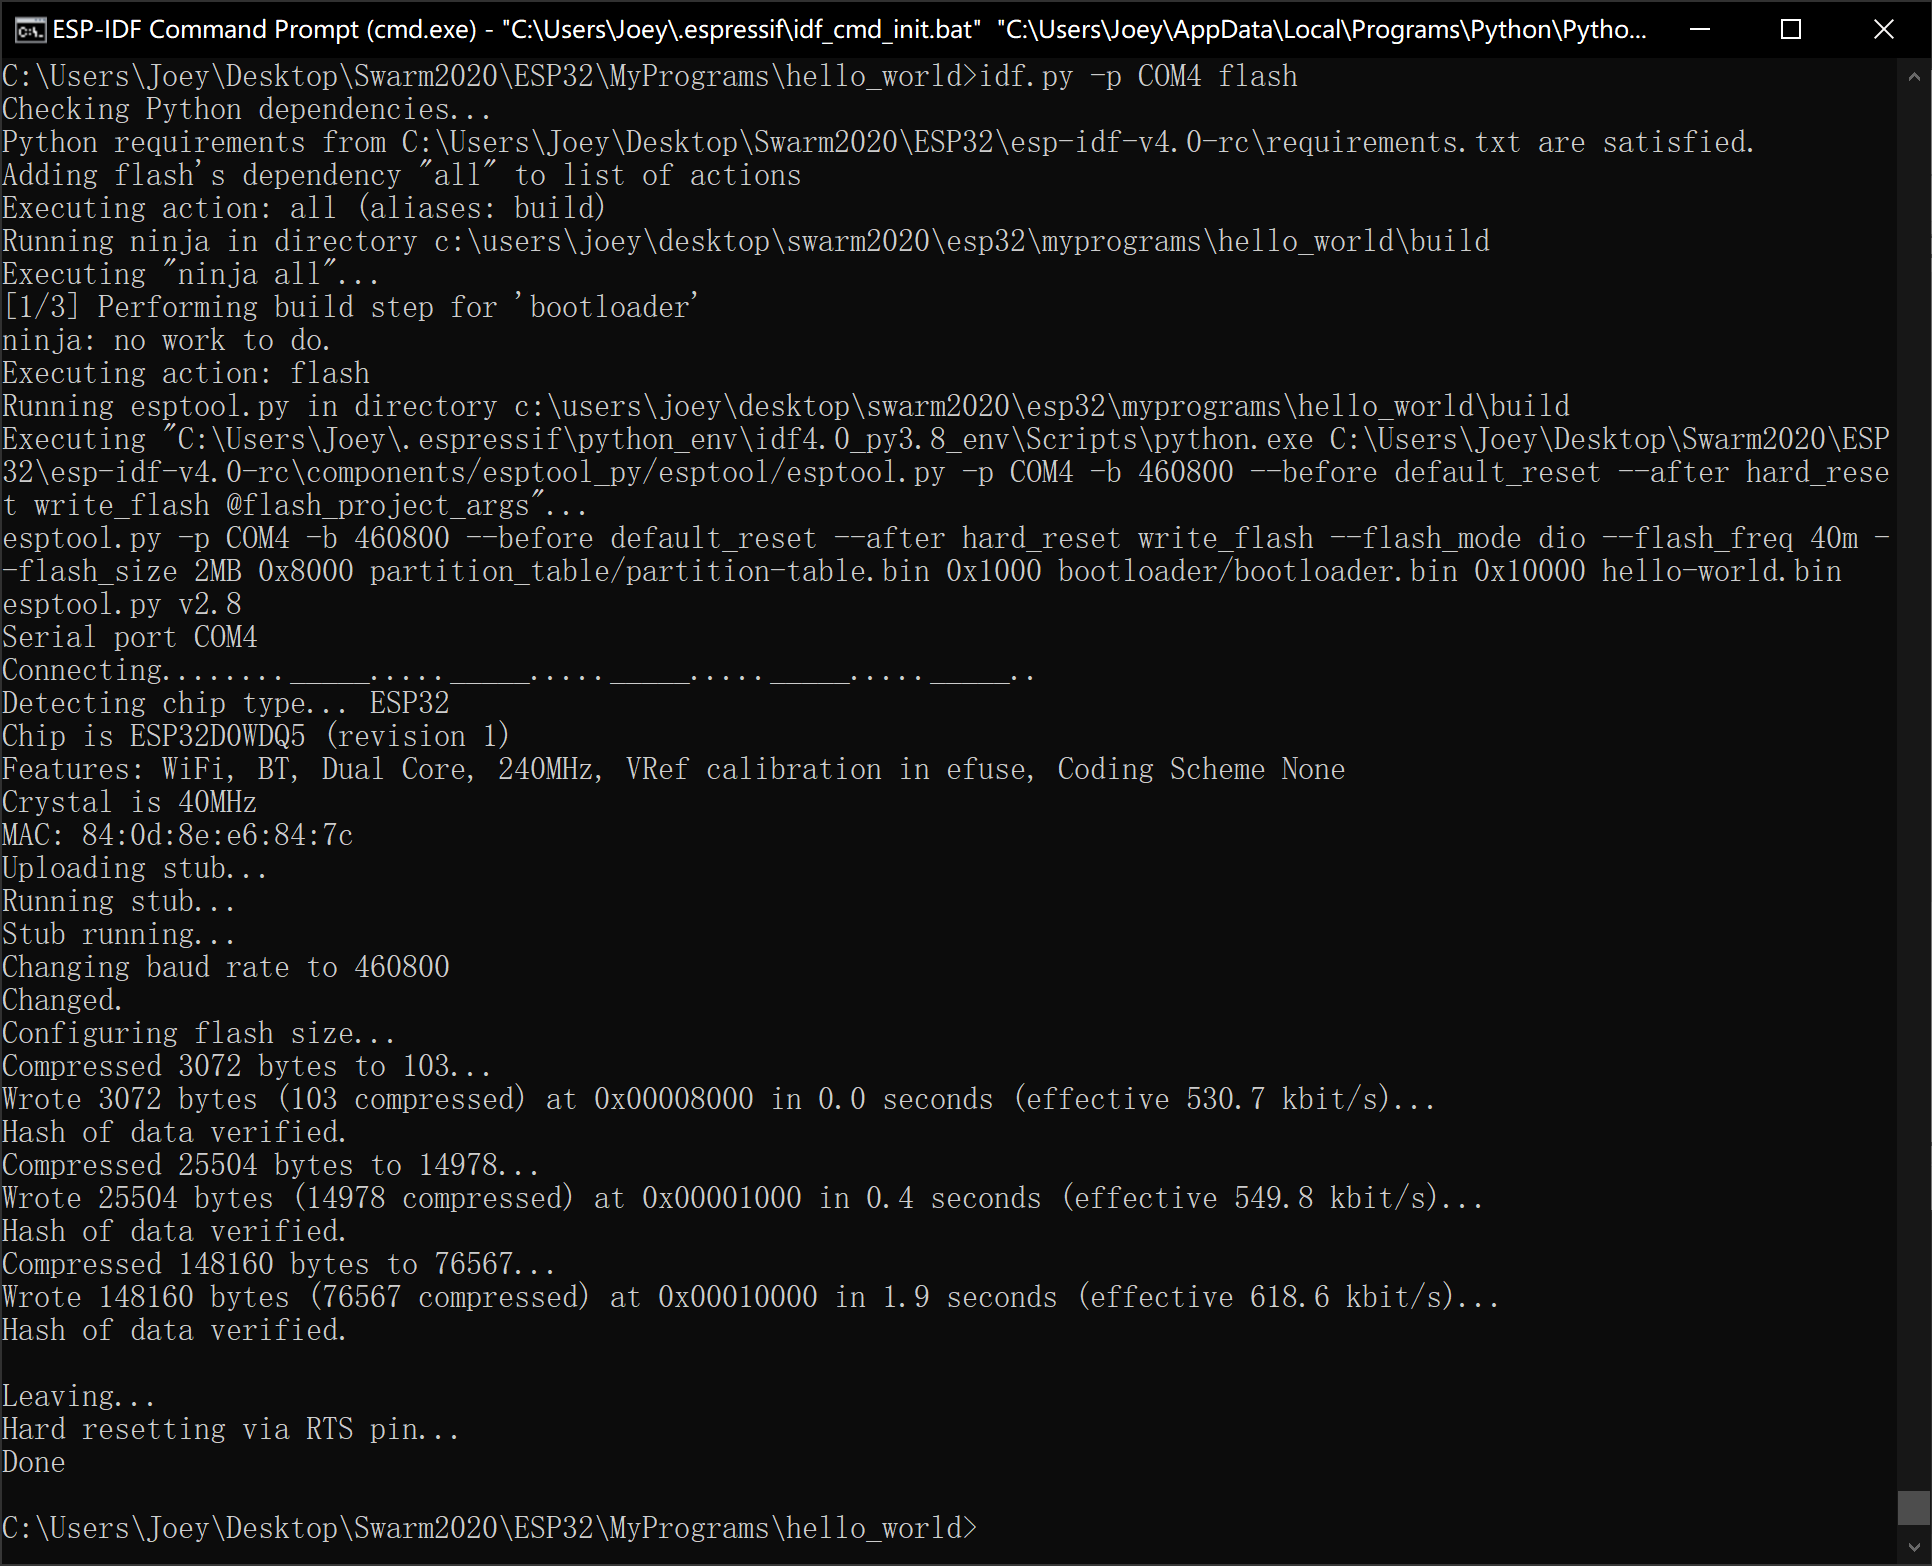
\includegraphics[width=\columnwidth]{ESP-IDF-Flash.png}
    \caption{ESP-IDF-Flash}
    \label{fig:ESP-IDF-Flash}
\end{figure}

\subsection{监视器}

可以使用 make monitor 命令,监视ESP32的运行情况。注意,不要忘记将 PORT 替换为串口名称。

也可以运行以下命令,一次性执行构建、烧录和监视过程:

\begin{tcolorbox}
    idf.py -p PORT flash monitor
\end{tcolorbox}

\begin{figure}[htbp]
    \centering
    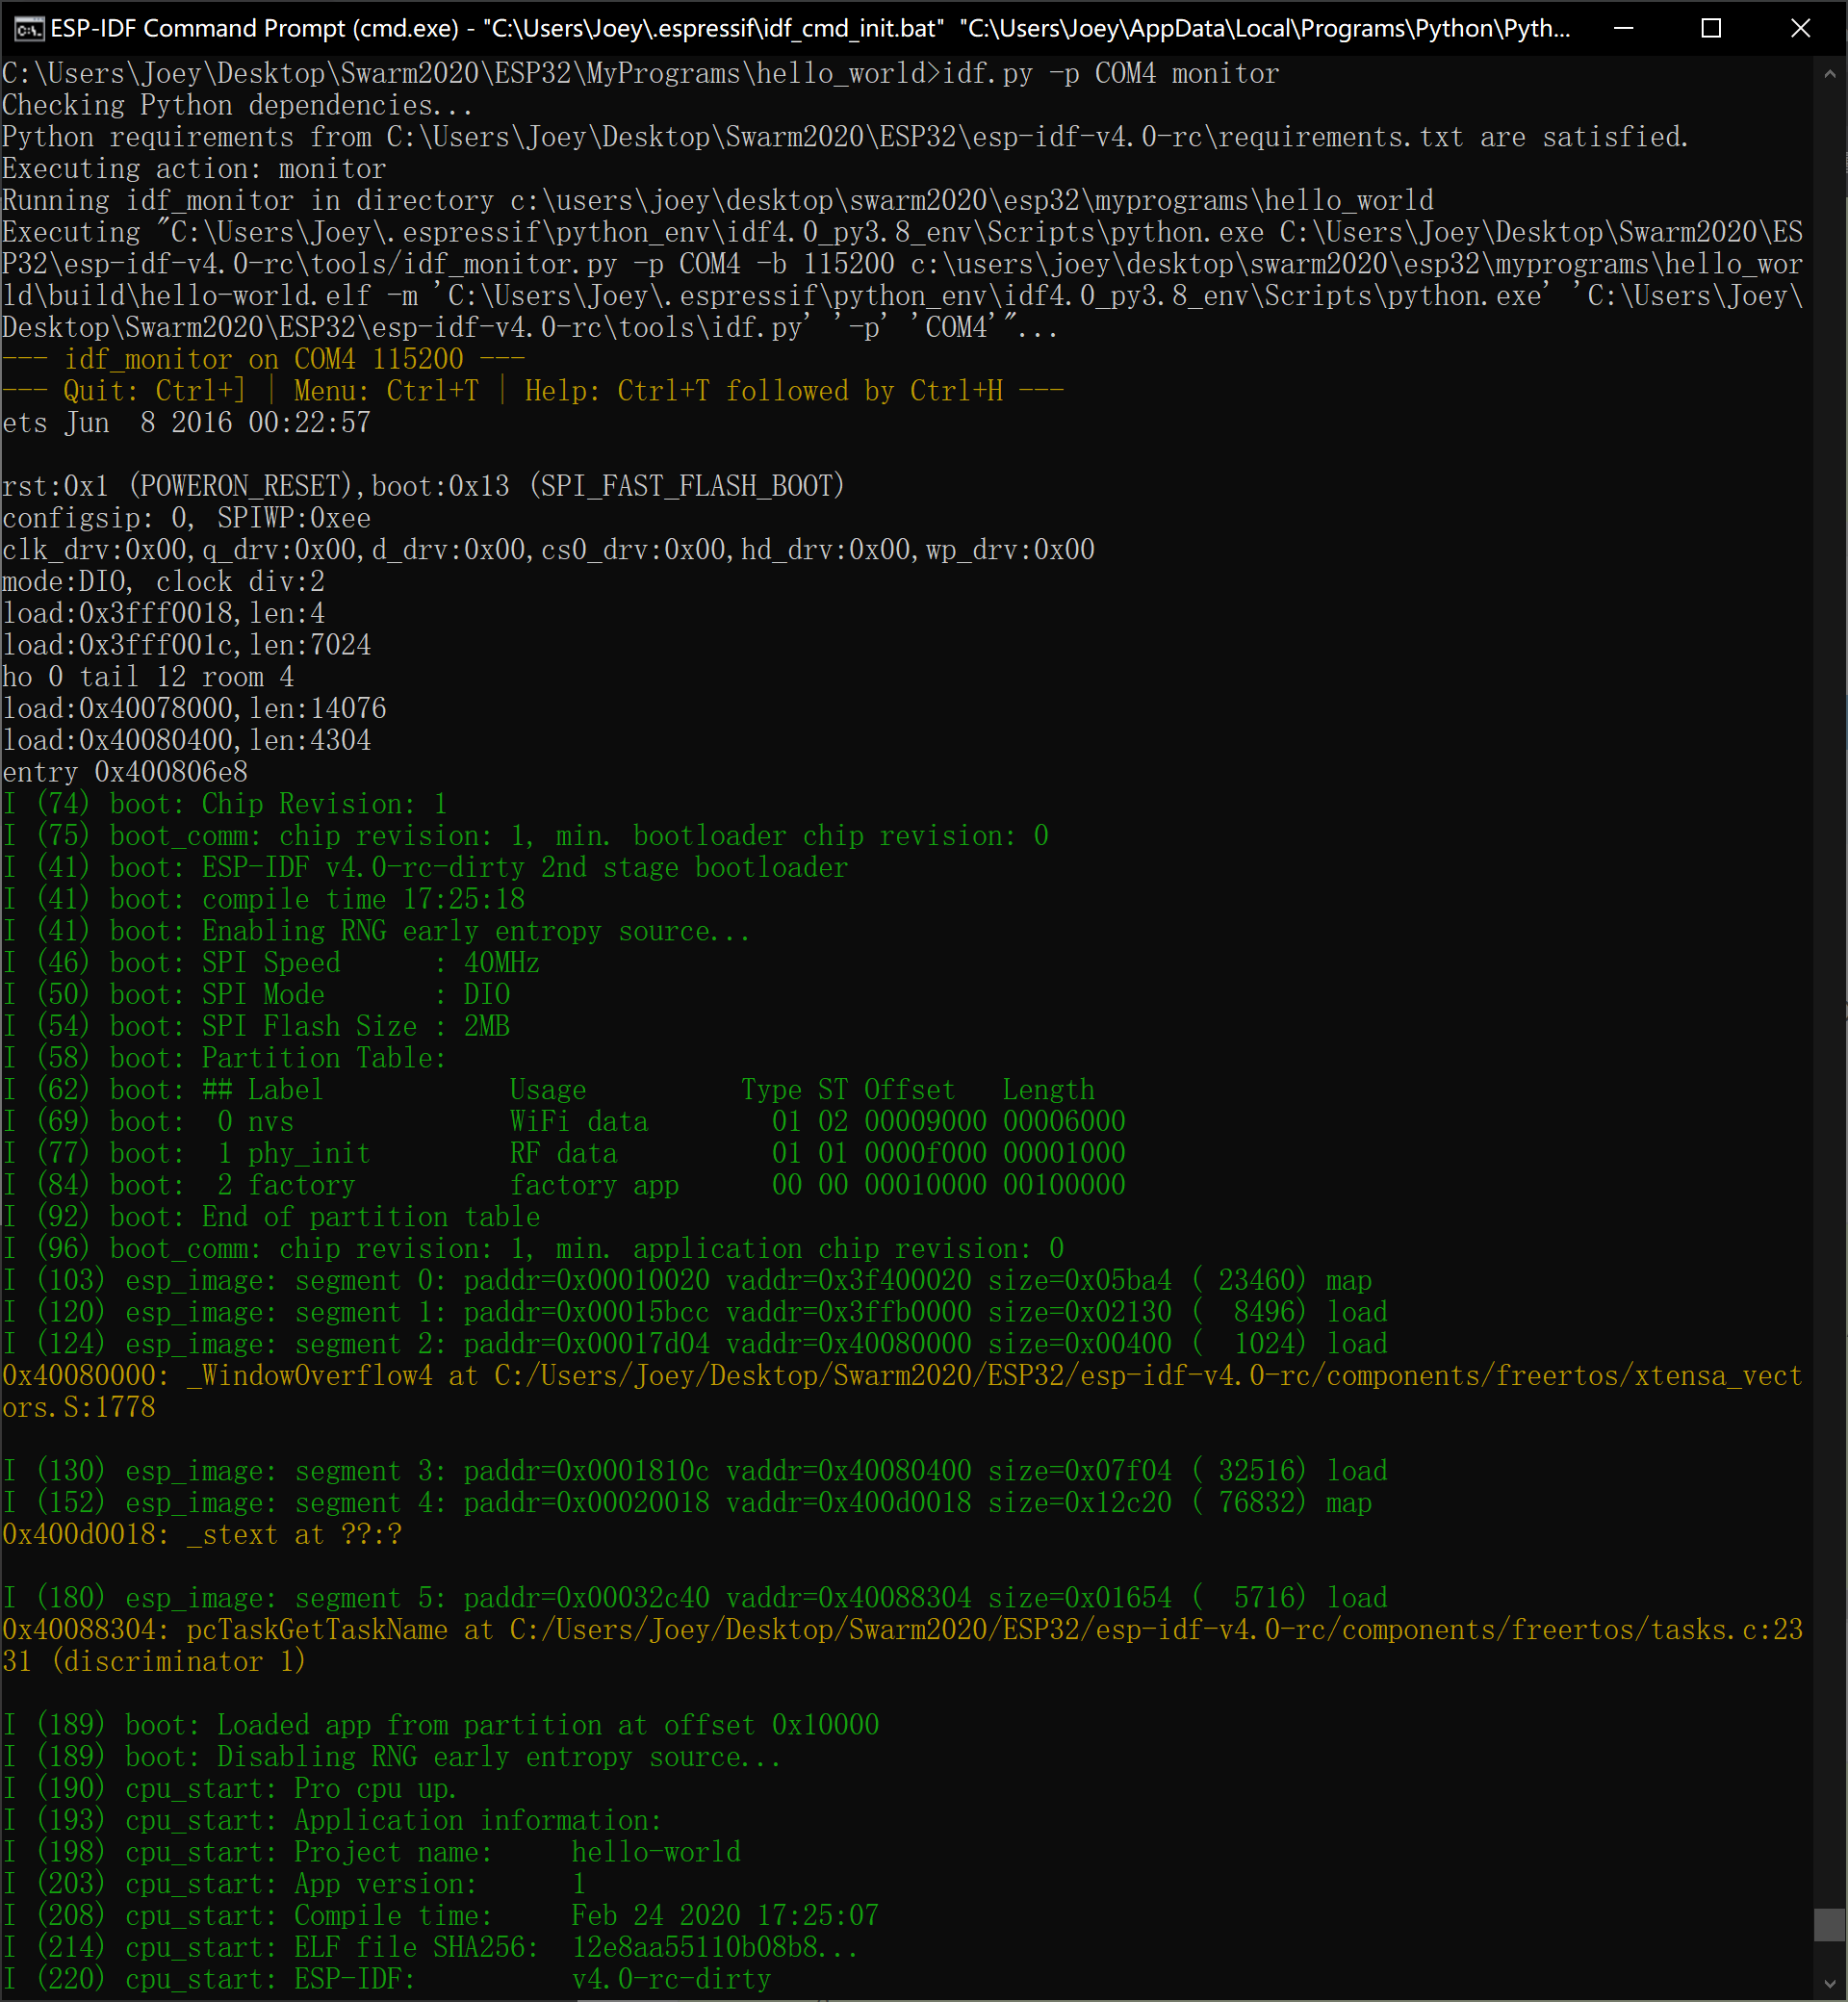
\includegraphics[width=\columnwidth]{ESP-IDF-Monitor-1.png}
    \caption{ESP-IDF-Monitor-1}
    \label{fig:ESP-IDF-Monitor-1}
\end{figure}

\begin{figure}[htbp]
    \centering
    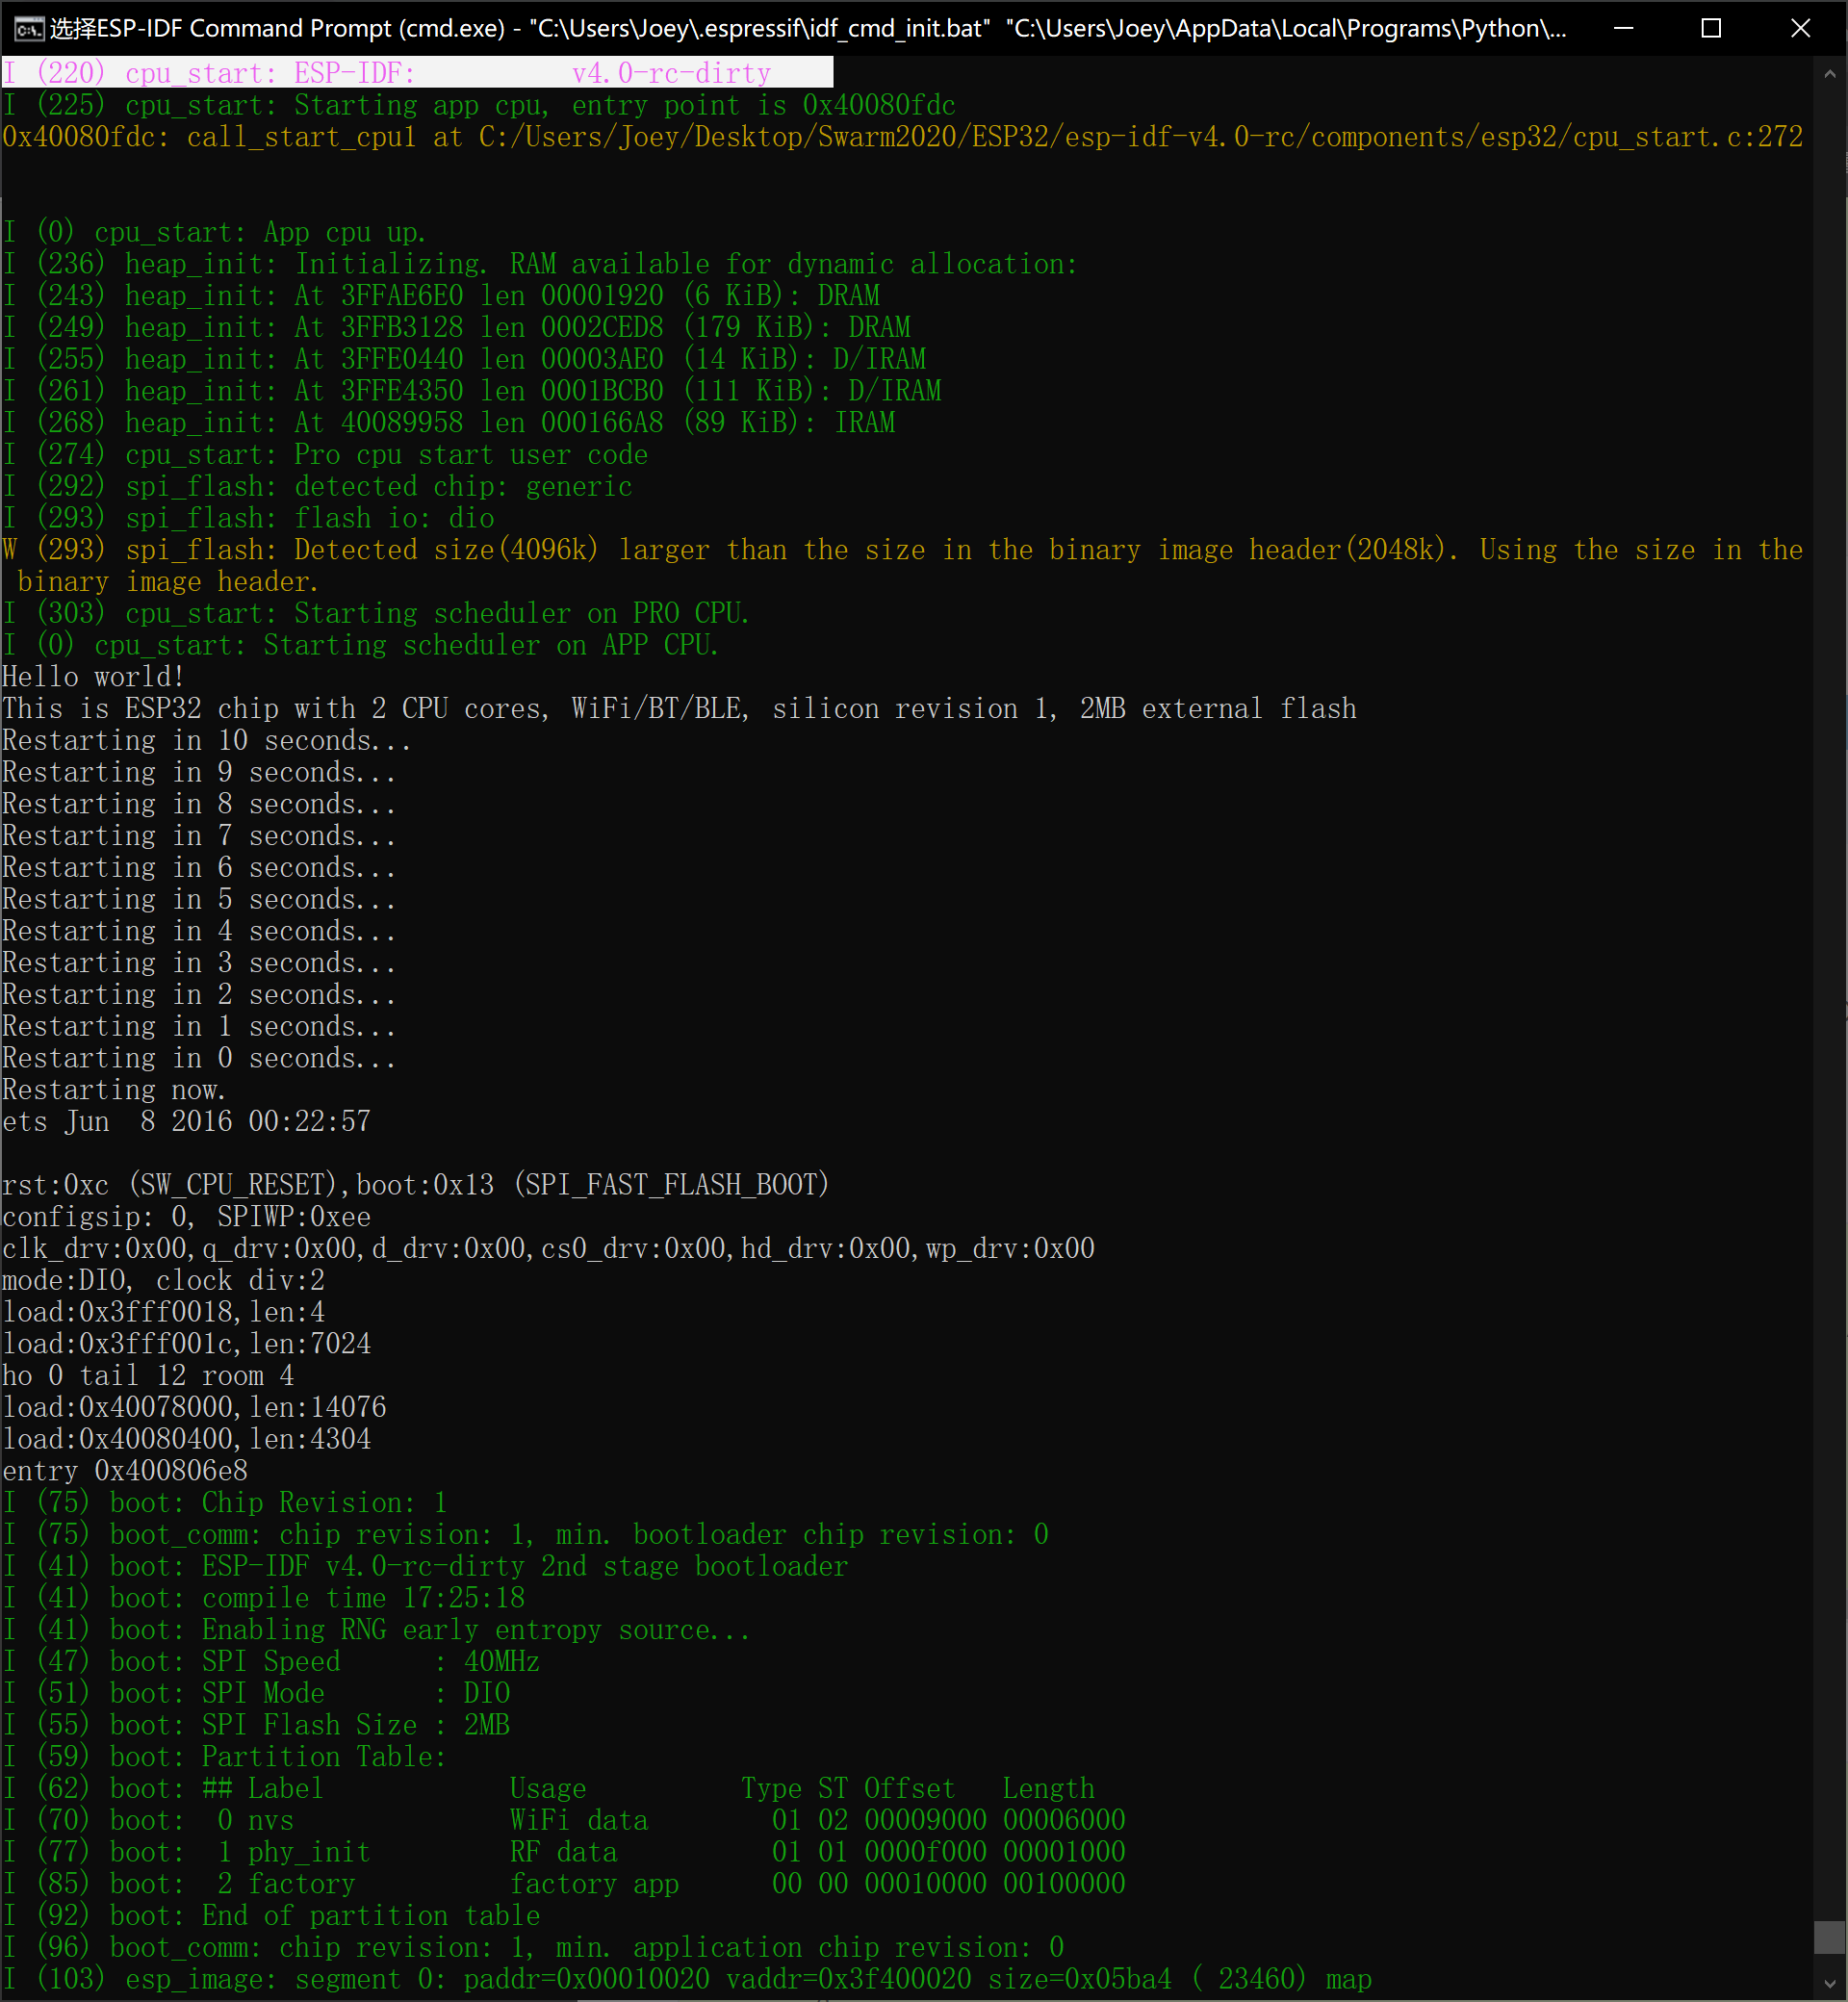
\includegraphics[width=\columnwidth]{ESP-IDF-Monitor-2.png}
    \caption{ESP-IDF-Monitor-2}
    \label{fig:ESP-IDF-Monitor-2}
\end{figure}

\begin{figure}[htbp]
    \centering
    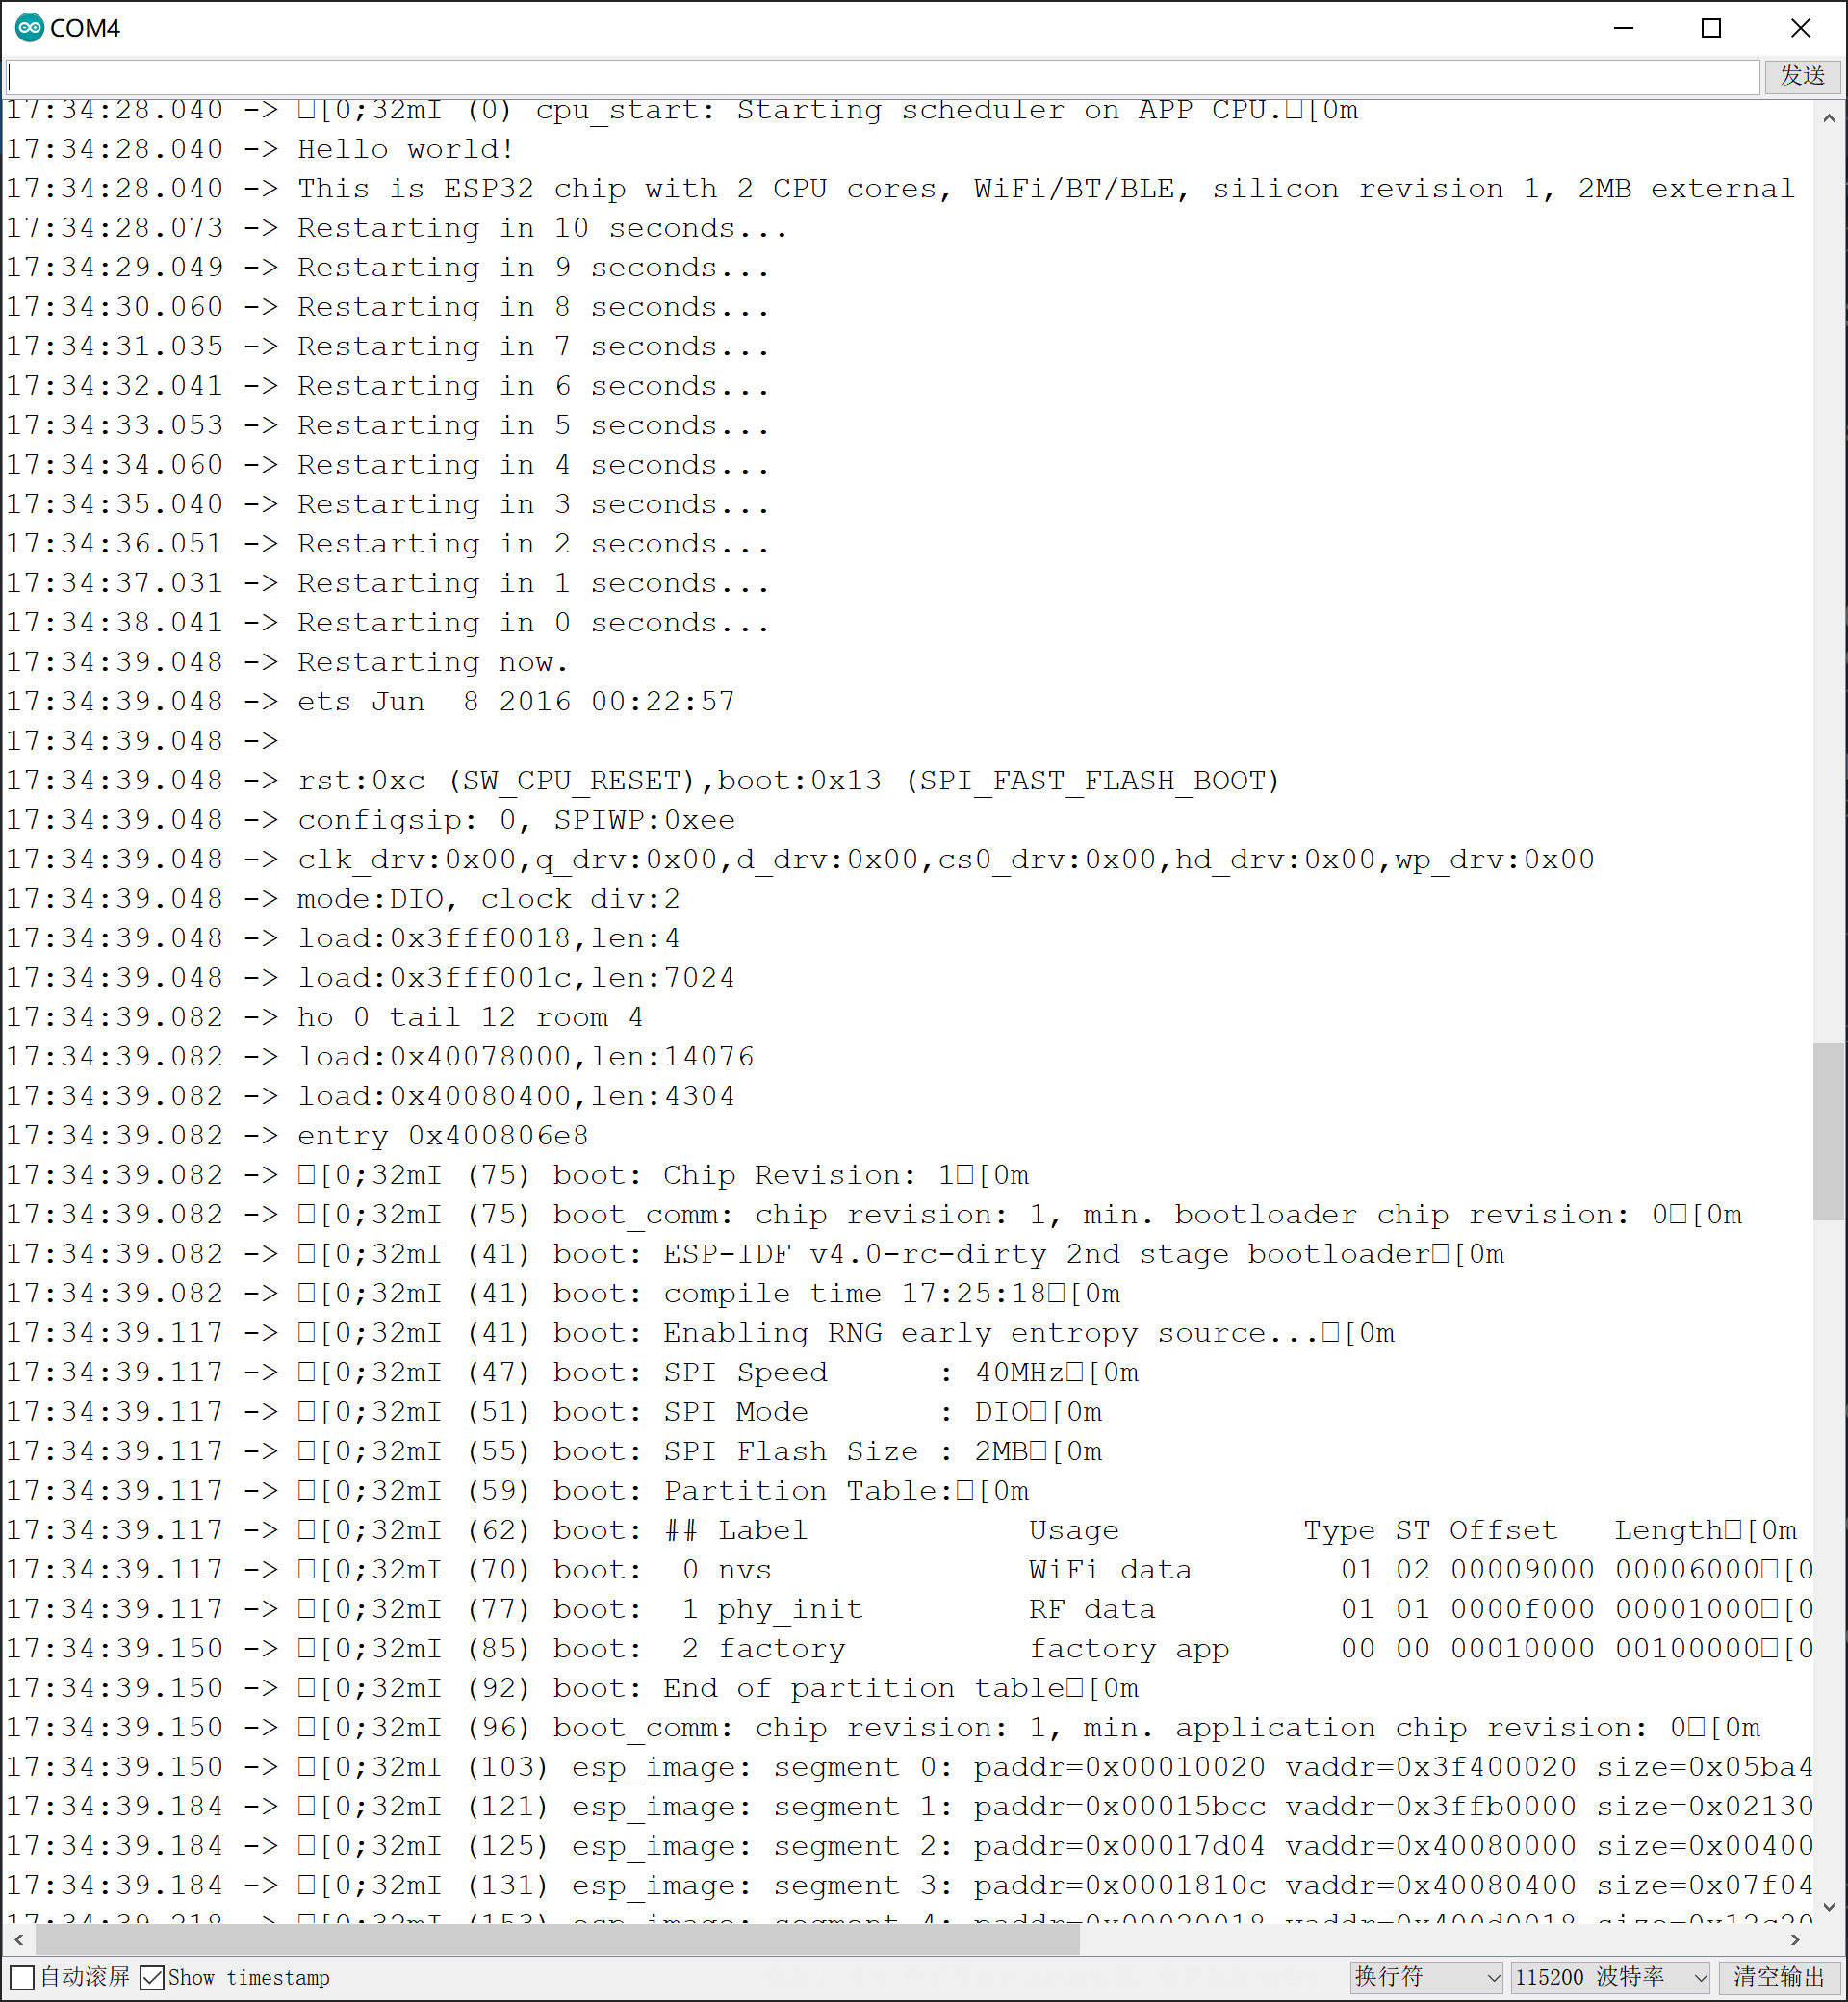
\includegraphics[width=\columnwidth]{ESP-IDF-Monitor-Arduino.png}
    \caption{ESP-IDF-Monitor-Arduino}
    \label{fig:ESP-IDF-Monitor-Arduino}
\end{figure}


\section{STM32开发环境}

STM32采用 Keil development development tools MDK-ARM Version 5.29 和 STM32CubeMX 配合进行程序设计。

STM32CubeMX 需要配合 64 位 Java 使用,在\url{https://java.com/zh_CN/download/manual.jsp}可以找到Windows 脱机 (64 位)安装exe。

\section{XBee环境}

Digi XCTU\footnote{\url{https://www.digi.com/xbee/software}} 提供了config的图形化界面。

\section{Python3.8环境配置}

安装Python时记得勾选初始页面下方的添加到PATH。

计算机上可能有多个版本的Python,在CMD中使用where python命令查看,在

VS Code中有Python插件,具体使用方法参考\url{https://code.visualstudio.com/docs/languages/python}。

注意左下角的Python interpreter要选成希望使用的版本对应的解释器,最好是PATH的第一个,防止出现pip包找不到的情况。Jupyter Notebook/Lab 同理。在我这台电脑上目前是Python 3.8.1 64-Bit,注意32bit 和 64bit Python的区别,它们用的是不同pip。

之后可以点右上角运行来执行脚本,和在Windows PowerShell里直接运行等价。

需要加断点看变量Debug可以使用VS Code左侧的Debug选项卡,根据向导创建一个launch.json,选Python-Python File即可。

\section{物理环境}

\begin{figure}[htbp]
    \centering
    \includegraphics[width=\columnwidth]{RealEnvironment1.jpg}
    \caption{焊接 贴片 环境}
    \label{fig:RealEnvironment1}
\end{figure}

\begin{figure}[htbp]
    \centering
    \includegraphics[width=\columnwidth]{RealEnvironment2.jpg}
    \caption{3D打印和装配环境}
    \label{fig:RealEnvironment2}
\end{figure}

\begin{figure}[htbp]
    \centering
    \includegraphics[width=\columnwidth]{RealEnvironment3.jpg}
    \caption{XBee通信调试环境}
    \label{fig:RealEnvironment3}
\end{figure}

% RealEnvironment1.jpg
% RealEnvironment2.jpg
% RealEnvironment3.jpg